\documentclass[10pt, a4paper]{report}
% !TeX program = xelatex
%==================PREAMBOLO=======================%
%%%%%%%%%%%%%%%%%%%%%%%%%%%%%%%%%%%%%%%%%%%%%%%%%%%%%%%%%%%%%%%%%%%%%%%%%%%%%
%% PREAMBLE
%% Reorganized for readability: packages, colors, custom commands, code
%% listing styles, tcolorbox theorem-like environments and title formatting
%% are grouped by purpose. No functional change was made to the original
%% document: only the order of declarations and the comments were edited.
%%%%%%%%%%%%%%%%%%%%%%%%%%%%%%%%%%%%%%%%%%%%%%%%%%%%%%%%%%%%%%%%%%%%%%%%%%%%%


%%%%%%%%%%%%%%%%%%%%%%%%%%%%%%%%%%%%%%%%%%%%%%%%%%%%%%%%%%%%%%%%%%%%%%%%%%%%%
%% 1. PACKAGES
%%%%%%%%%%%%%%%%%%%%%%%%%%%%%%%%%%%%%%%%%%%%%%%%%%%%%%%%%%%%%%%%%%%%%%%%%%%%%

% --- Encoding, language and fonts ---------------------------------------
\usepackage[utf8]{inputenc}
\usepackage[T1]{fontenc}
\usepackage[english]{babel}
\usepackage{mathpazo}          % Palatino font, replaces lmodern to match the image's serif style
\usepackage[scaled]{helvet}    % Helvetica, used for section/subsection titles

% --- Page layout and headers/footers ------------------------------------
\usepackage[paper=a4paper,left=25mm,right=25mm,bottom=25mm,top=25mm]{geometry}
\usepackage{fancyhdr}
\usepackage[Rejne]{fncychap}
\usepackage{titlesec}
\usepackage{titletoc}
\usepackage{needspace}

% --- Math ----------------------------------------------------------------
\usepackage{amsmath}
\usepackage{amssymb}
\usepackage{amsfonts}
\usepackage{mathtools}
\usepackage{mathrsfs}
\usepackage{stmaryrd}
\usepackage{nicefrac, xfrac}

% --- Graphics and TikZ -----------------------------------------------------
\usepackage{graphicx}          % Required for inserting images
\usepackage[export]{adjustbox}
\usepackage{pdfpages}
\usepackage{tikz}
\usepackage{tikz-3dplot}
\usepackage{tikz-cd}
\usepackage{pgfplots}
\usepackage{pgf-pie}
\usetikzlibrary{positioning}

% --- Colors and colored boxes ---------------------------------------------
\usepackage[table,xcdraw]{xcolor}
\usepackage[most]{tcolorbox}
\tcbuselibrary{theorems}

% --- Lists, layout helpers and decorations --------------------------------
\usepackage[shortlabels]{enumitem}
\usepackage{wrapfig}
\usepackage{multicol}
\usepackage{moresize}
\usepackage{fourier-orns}       % Decorative ornaments (used by \flowerLine, \eqImportante)
\usepackage{psvectorian}        % Decorative vectorial ornaments
\usepackage{lipsum}             % Placeholder ("dummy") text
\usepackage{blindtext}          % Placeholder ("dummy") text

% --- Code listings ---------------------------------------------------------
\usepackage{listings}
\usepackage{minted}

% --- Miscellaneous ---------------------------------------------------------
\usepackage{hyperref}


%%%%%%%%%%%%%%%%%%%%%%%%%%%%%%%%%%%%%%%%%%%%%%%%%%%%%%%%%%%%%%%%%%%%%%%%%%%%%
%% 2. COLOR DEFINITIONS
%%%%%%%%%%%%%%%%%%%%%%%%%%%%%%%%%%%%%%%%%%%%%%%%%%%%%%%%%%%%%%%%%%%%%%%%%%%%%

% --- General purpose colors ---
\definecolor{light-gray}{gray}{0.95}
\definecolor{darkgreen}{HTML}{008000}
\definecolor{g}{RGB}{60, 50, 50}

% --- "Sapienza" theme colors ---
\definecolor{sapienza}{HTML}{660f1d}
\definecolor{lightSapienza}{HTML}{e3d3d5}

% --- Cover / decorative colors ---
\definecolor{cop}{HTML}{f7ecd7}
\definecolor{copAut}{HTML}{ababab}
\definecolor{copAut2}{HTML}{c3c3e6}
\definecolor{purcop}{HTML}{d0d3db}
\definecolor{cartaRiciclata}{HTML}{fcfcf7}

% --- Colors used for C / C++ code listings ---
\definecolor{mGreen}{rgb}{0,0.6,0}
\definecolor{mGray}{rgb}{0.5,0.5,0.5}
\definecolor{mPurple}{rgb}{0.58,0,0.82}
\definecolor{backgroundColour}{rgb}{0.95,0.95,0.92}


%%%%%%%%%%%%%%%%%%%%%%%%%%%%%%%%%%%%%%%%%%%%%%%%%%%%%%%%%%%%%%%%%%%%%%%%%%%%%
%% 3. CUSTOM COMMANDS
%%%%%%%%%%%%%%%%%%%%%%%%%%%%%%%%%%%%%%%%%%%%%%%%%%%%%%%%%%%%%%%%%%%%%%%%%%%%%

% --- Colored text shortcuts ------------------------------------------------
\newcommand{\redText}[1]{\color{red}#1\color{black}}
\newcommand{\blueText}[1]{\color{blue}#1\color{black}}
\newcommand{\greenText}[1]{\color{darkgreen}#1\color{black}}
\newcommand{\sapText}[1]{\color{sapienza}#1\color{black}}
\newcommand{\textg}[1]{\color{g}{\textbf{#1}}\color{black}}

% --- Inline code / shell snippets -------------------------------------------
\newcommand{\code}[1]{\colorbox{light-gray}{\texttt{#1}}}
\newcommand{\codee}[1]{\colorbox{white}{\texttt{#1}}}
\newcommand{\shell}[1]{\colorbox{black}{\textcolor{white}{\texttt{#1}}}}
\newcommand{\boxedMath}[1]{\begin{tabular}{|c|}\hline \texttt{#1} \\ \hline\end{tabular} :}

% --- Highlighted paragraph boxes --------------------------------------------
\newcommand\greybox[1]{%
  \vskip\baselineskip%
  \par\noindent\colorbox{light-gray}{%
    \begin{minipage}{\textwidth}#1\end{minipage}%
  }%
  \vskip\baselineskip%
}
\newcommand\sapbox[1]{%
  \vskip\baselineskip%
  \par\noindent\colorbox{lightSapienza}{%
    \begin{minipage}{\textwidth}#1\end{minipage}%
  }%
  \vskip\baselineskip%
}

% --- Statement labels (theorem/definition/etc. headers as plain text) ------
\newcommand{\teo}[1]{{\large\color{sapienza}\textbf{Teorema #1 :\hphantom{a}}}}
\newcommand{\defi}[1]{{\large\color{sapienza}\textbf{Definizione #1 :\hphantom{a}}}}
\newcommand{\prop}[1]{{\color{sapienza}\textbf{Proposizione #1 :\hphantom{a}}}}
\newcommand{\lemma}[1]{{\color{sapienza}\textbf{Lemma #1 :\hphantom{a}}}}
\newcommand{\claim}[1]{{\color{sapienza}\textbf{Claim #1 :\hphantom{a}}}}
\newcommand{\dimo}[1]{{\color{sapienza}\textbf{Dimostrazione #1 :\hphantom{a}}}}
\newcommand{\acc}{\\\hphantom{}\\}
\newcommand{\esempio}[1]{{\acc\large\color{sapienza}\textbf{Esempio #1 \hphantom{a}}\acc}}

% --- Number sets and blackboard-bold symbols --------------------------------
\newcommand{\N}{{\mathbb N}}
\newcommand{\Z}{{\mathbb Z}}
\newcommand{\R}{{\mathbb R}}
\newcommand{\C}{{\mathbb C}}
\newcommand{\K}{{\mathbb K}}
\newcommand{\quat}{{\mathbb H}}
\newcommand{\Prob}{{\mathbb P}}
\newcommand{\VA}{{\mathbb E}}

% --- Calligraphic / script symbols ------------------------------------------
\newcommand{\Sn}{{\mathcal S_n}}
\newcommand{\An}{{\mathcal A_n}}
\newcommand{\E}{{\mathcal E}}
\newcommand{\B}{{\mathcal B}}

% --- Bold vector/greek symbols ----------------------------------------------
\newcommand{\btheta}{{\boldsymbol{\theta}}}
\newcommand{\btau}{{\boldsymbol{\tau}}}
\newcommand{\bomega}{{\boldsymbol{\omega}}}
\newcommand{\Bomega}{{\boldsymbol{\Omega}}}
\newcommand{\bmu}{{\boldsymbol{\mu}}}
\newcommand{\brho}{{\boldsymbol{\rho}}}
\newcommand{\bnu}{{\boldsymbol{\nu}}}
\newcommand{\bsigma}{{\boldsymbol{\sigma}}}
\newcommand{\blambda}{{\boldsymbol{\lambda}}}

% --- Dotted mechanics symbols (velocity/acceleration notation) -------------
\newcommand{\dq}{{\dot{\mathbf q}}}
\newcommand{\de}{{\dot{\mathbf e}}}
\newcommand{\dy}{{\dot{\mathbf y}}}
\newcommand{\ddq}{{\ddot{\mathbf q}}}
\newcommand{\ddy}{{\ddot{\mathbf y}}}
\newcommand{\ve}{{\bar v}}

% --- Group theory / algebra operators ---------------------------------------
\newcommand{\aut}{{\text{Aut}}}
\newcommand{\Span}{{\text{Span}}}
\newcommand{\End}{{\text{End}}}
\newcommand{\cen}{{\text{Centro}}}
\newcommand{\norm}{{\unlhd}}
\newcommand{\ciclS}{{\left \langle }}
\newcommand{\ciclE}{{\right \rangle }}
\newcommand{\bra}[1]{\langle #1 \rangle}
\newcommand{\mcm}{{\text{mcm}}}
\newcommand{\MCD}{{\text{MCD}}}
\newcommand{\rg}{{\text{rg}}}
\newcommand{\supp}{{\text{Supp}}}

% --- Complexity theory symbols -----------------------------------------------
\newcommand{\ridFunc}{{f:\Sigma^*\rightarrow \Sigma^*}}
\newcommand{\rid}{{\le_m^P}}
\newcommand{\blank}{{\sqcup}}

% --- Miscellaneous math symbols and utilities -------------------------------
\newcommand{\quadBrack}[1]{ \llbracket #1 \rrbracket }
\newcommand{\notimplies}{%
  \mathrel{{\ooalign{\hidewidth$\not\phantom{=}$\hidewidth\cr$\implies$}}}}
\newcommand{\tc}{{\text{ tale che }}}
\newcommand{\spaz}{{\text{\hphantom{aa}}}}

% --- Decorative separators ---------------------------------------------------
\newcommand{\flowerLine}{ \begin{center}\decofourleft\hphantom{ }\decoone\hphantom{ }\decofourright\hphantom{}\hphantom{aa}
\decofourleft\hphantom{ }\decoone\hphantom{ }\decofourright\hphantom{}\hphantom{aa}
\decofourleft\hphantom{ }\decoone\hphantom{ }\decofourright\hphantom{}\hphantom{aa}
\decofourleft\hphantom{ }\decoone\hphantom{ }\decofourright\hphantom{}\hphantom{aa} 
\decofourleft\hphantom{ }\decoone\hphantom{ }\decofourright\hphantom{}\hphantom{aa}
\decofourleft\hphantom{ }\decoone\hphantom{ }\decofourright\hphantom{}\hphantom{aa}
\decofourleft\hphantom{ }\decoone\hphantom{ }\decofourright\hphantom{}\hphantom{aa}
\decofourleft\hphantom{ }\decoone\hphantom{ }\decofourright\hphantom{}\hphantom{aa}
\decofourleft\hphantom{ }\decoone\hphantom{ }\decofourright\hphantom{}\hphantom{aa}
\end{center}}
\newcommand{\eqImportante}[1]{\begin{center}\huge\lefthand\hphantom{a}
    \normalsize\texttt{#1}
    \hphantom{aaa}\huge\righthand\end{center}}


%%%%%%%%%%%%%%%%%%%%%%%%%%%%%%%%%%%%%%%%%%%%%%%%%%%%%%%%%%%%%%%%%%%%%%%%%%%%%
%% 4. PAGE STYLE (HEADER / FOOTER)
%%%%%%%%%%%%%%%%%%%%%%%%%%%%%%%%%%%%%%%%%%%%%%%%%%%%%%%%%%%%%%%%%%%%%%%%%%%%%
\fancyhf{}
\pagestyle{fancy}
\renewcommand{\headrulewidth}{0.4pt}


%%%%%%%%%%%%%%%%%%%%%%%%%%%%%%%%%%%%%%%%%%%%%%%%%%%%%%%%%%%%%%%%%%%%%%%%%%%%%
%% 5. CODE LISTING STYLES (C / C++)
%%%%%%%%%%%%%%%%%%%%%%%%%%%%%%%%%%%%%%%%%%%%%%%%%%%%%%%%%%%%%%%%%%%%%%%%%%%%%
% The following styles configure the `listings` package for displaying
% C and C++ source code with syntax highlighting.

\lstdefinestyle{CStyle}{
    backgroundcolor=\color{backgroundColour},   
    commentstyle=\color{mGreen},
    keywordstyle=\color{magenta},
    numberstyle=\tiny\color{mGray},
    stringstyle=\color{mPurple},
    basicstyle=\footnotesize,
    breakatwhitespace=false,         
    breaklines=true,                 
    captionpos=b,                    
    keepspaces=true,                 
    numbers=left,                    
    numbersep=5pt,                  
    showspaces=false,                
    showstringspaces=false,
    showtabs=false,                  
    tabsize=2,
    language=C
}

\lstdefinestyle{CppStyle}{
    backgroundcolor=\color{backgroundColour},   
    commentstyle=\color{mGreen}\ttfamily,
    morecomment=[l][\color{magenta}]{\#}
    keywordstyle=\color{blue}\ttfamily,
    numberstyle=\tiny\color{mGray},
    stringstyle=\color{red}\ttfamily,
    basicstyle=\ttfamily,
    breakatwhitespace=false,         
    breaklines=true,                 
    captionpos=b,                    
    keepspaces=true,                 
    numbers=left,                    
    numbersep=5pt,                  
    showspaces=false,                
    showstringspaces=false,
    showtabs=false,                  
    tabsize=2,
    language=C
}

% Global default `listings` configuration (applied when no style is selected)
\lstset{language=C++,
                basicstyle=\ttfamily,
                keywordstyle=\color{blue}\ttfamily,
                stringstyle=\color{red}\ttfamily,
                commentstyle=\color{green}\ttfamily,
                morecomment=[l][\color{magenta}]{\#}
}


%%%%%%%%%%%%%%%%%%%%%%%%%%%%%%%%%%%%%%%%%%%%%%%%%%%%%%%%%%%%%%%%%%%%%%%%%%%%%
%% 6. TCOLORBOX THEOREM-LIKE ENVIRONMENTS
%%%%%%%%%%%%%%%%%%%%%%%%%%%%%%%%%%%%%%%%%%%%%%%%%%%%%%%%%%%%%%%%%%%%%%%%%%%%%
% Each environment below renders a boxed, numbered statement (definition,
% theorem, proposition, ...) with a "tab" style title in the top-left
% corner, following the same visual template.

\newtcbtheorem[number within=section]{boxdefinition}{Definition}{
    enhanced,
    before skip=15pt, after skip=15pt,
    colback=white,                          % white background for the text
    colframe=sapienza!50!black!30,          % border color (light green/gray)
    fonttitle=\bfseries,
    coltitle=black,
    % Style of the top-left "tab"
    attach boxed title to top left={xshift=10mm, yshift=-3.5mm, yshifttext=-1mm},
    boxed title style={
        colframe=sapienza!50!black!30,
        arc=3mm,
        outer arc=3mm,
        left=10pt, right=10pt,
        top=2pt, bottom=2pt,
        % Green gradient shading, as in the reference image
        interior style={left color=sapienza!20, right color=sapienza!40}
    },
    % Rounding of the main box
    arc=4mm,
    separator sign none,                    % removes the automatic colon so it can be added manually in the title
    description font=\normalfont\bfseries,
    description delimiters={: }{ }          % formats the title as "Definition 2.1: Title"
}{def}

\newtcbtheorem[number within=section]{boxtheorem}{Theorem}{
    enhanced,
    before skip=15pt, after skip=15pt,
    colback=white,
    colframe=sapienza!50!black!30,
    fonttitle=\bfseries,
    coltitle=black,
    attach boxed title to top left={xshift=10mm, yshift=-3.5mm, yshifttext=-1mm},
    boxed title style={
        colframe=sapienza!50!black!30,
        arc=3mm,
        outer arc=3mm,
        left=10pt, right=10pt,
        top=2pt, bottom=2pt,
        interior style={left color=sapienza!20, right color=sapienza!40}
    },
    arc=4mm,
    separator sign none,
    description font=\normalfont\bfseries,
    description delimiters={: }{ }
}{def}

\newtcbtheorem[number within=section]{boxproposition}{Proposition}{
    enhanced,
    before skip=15pt, after skip=15pt,
    colback=white,
    colframe=sapienza!50!black!30,
    fonttitle=\bfseries,
    coltitle=black,
    attach boxed title to top left={xshift=10mm, yshift=-3.5mm, yshifttext=-1mm},
    boxed title style={
        colframe=sapienza!50!black!30,
        arc=3mm,
        outer arc=3mm,
        left=10pt, right=10pt,
        top=2pt, bottom=2pt,
        interior style={left color=sapienza!30, right color=sapienza!50}
    },
    arc=4mm,
    separator sign none,
    description font=\normalfont\bfseries,
    description delimiters={: }{ }
}{def}

\newtcbtheorem[number within=section]{boxequation}{Equation}{
    enhanced,
    before skip=15pt, after skip=15pt,
    colback=white,
    colframe=sapienza!50!black!30,
    fonttitle=\bfseries,
    coltitle=black,
    attach boxed title to top left={xshift=10mm, yshift=-3.5mm, yshifttext=-1mm},
    boxed title style={
        colframe=sapienza!50!black!30,
        arc=3mm,
        outer arc=3mm,
        left=10pt, right=10pt,
        top=2pt, bottom=2pt,
        interior style={left color=sapienza!30, right color=sapienza!50}
    },
    arc=4mm,
    separator sign none,
    description font=\normalfont\bfseries,
    description delimiters={: }{ }
}{def}

\newtcbtheorem[number within=section]{boxlemma}{Lemma}{
    enhanced,
    before skip=15pt, after skip=15pt,
    colback=white,
    colframe=sapienza!50!black!30,
    fonttitle=\bfseries,
    coltitle=black,
    attach boxed title to top left={xshift=10mm, yshift=-3.5mm, yshifttext=-1mm},
    boxed title style={
        colframe=sapienza!50!black!30,
        arc=3mm,
        outer arc=3mm,
        left=10pt, right=10pt,
        top=2pt, bottom=2pt,
        interior style={left color=sapienza!30, right color=sapienza!50}
    },
    arc=4mm,
    separator sign none,
    description font=\normalfont\bfseries,
    description delimiters={: }{ }
}{def}

\newtcbtheorem[number within=section]{boxobservation}{Observation}{
    enhanced,
    before skip=15pt, after skip=15pt,
    colback=white,
    colframe=sapienza!50!black!30,
    fonttitle=\bfseries,
    coltitle=black,
    attach boxed title to top left={xshift=10mm, yshift=-3.5mm, yshifttext=-1mm},
    boxed title style={
        colframe=sapienza!50!black!30,
        arc=3mm,
        outer arc=3mm,
        left=10pt, right=10pt,
        top=2pt, bottom=2pt,
        interior style={left color=sapienza!30, right color=sapienza!50}
    },
    arc=4mm,
    separator sign none,
    description font=\normalfont\bfseries,
    description delimiters={: }{ }
}{def}

\newtcbtheorem[number within=section]{boxpostulate}{Postulate}{
    enhanced,
    before skip=15pt, after skip=15pt,
    colback=white,
    colframe=sapienza!50!black!30,
    fonttitle=\bfseries,
    coltitle=black,
    attach boxed title to top left={xshift=10mm, yshift=-3.5mm, yshifttext=-1mm},
    boxed title style={
        colframe=sapienza!50!black!30,
        arc=3mm,
        outer arc=3mm,
        left=10pt, right=10pt,
        top=2pt, bottom=2pt,
        interior style={left color=sapienza!30, right color=sapienza!50}
    },
    arc=4mm,
    separator sign none,
    description font=\normalfont\bfseries,
    description delimiters={: }{ }
}{def}


%%%%%%%%%%%%%%%%%%%%%%%%%%%%%%%%%%%%%%%%%%%%%%%%%%%%%%%%%%%%%%%%%%%%%%%%%%%%%
%% 7. SECTION / SUBSECTION TITLE FORMATTING
%%%%%%%%%%%%%%%%%%%%%%%%%%%%%%%%%%%%%%%%%%%%%%%%%%%%%%%%%%%%%%%%%%%%%%%%%%%%%

% Section titles: Helvetica, large bold number, colored rule underneath
\titleformat{\section}
  {\needspace{3\baselineskip} % requires at least 3 lines of free space before the title
   \fontfamily{phv}\selectfont\huge\bfseries} 
  {\color{sapienza}\fontsize{20}{20}\selectfont\thesection} 
  {12pt} 
  {} 
  [\vspace{2pt}\nopagebreak\color{sapienza!40}\hrule height 3pt]

% Subsection titles: same style, slightly smaller
\titleformat{\subsection}
  {\needspace{2\baselineskip} % requires at least 2 lines of free space before the title
   \fontfamily{phv}\selectfont\Large\bfseries} 
  {\color{sapienza}\fontsize{16}{16}\selectfont\thesubsection} 
  {12pt} 
  {} 
  [\vspace{2pt}\nopagebreak\color{sapienza!40}\hrule height 1.5pt]
\newcommand{\y}{{\mathbf y}}
\newcommand{\q}{{\mathbf q}}
\usepackage{algorithm}
\usepackage{algpseudocode}
 \usepackage{multirow}
\newcommand{\titolo}{Reinforcement Learning}

 %TOGLI COMMENTO SE USI XELATEX
%\usepackage{fontspec}
\title{\titolo} %========TITOLO========%
\author{Marco Casu}
\date{\vspace{-5ex}}
\begin{document}

%==================COPERTINA=======================%
\begin{titlepage}
    \centering
     
    
\includegraphics[width=0.6\textwidth]{../../preamble/Stemma_sapienza.png} 
    \par\vspace{2.5cm}
    
    {\huge \textsc{``Sapienza'' University of Rome}}
    \par\vspace{0.5cm}
    {\Large \textsc{Faculty of Information Engineering,\\ Computer Science and Statistics}} \\[1.5ex]
    {\Large \textsc{Department of Computer, Control\\ and Management Engineering}}
    \\[1.5ex]
    {\Large \textsc{Master's degree in Artificial Intelligence and Robotics
}}
    
    \vspace{2.5cm} % Spazio verticale regolabile
    
    \rule{\textwidth}{2pt} \\
    \vspace{0.5cm}
    {\fontsize{35}{70} \selectfont \textbf{\titolo}} \\
    \vspace{0.35cm}
    \rule{\textwidth}{2pt}
    
    \vspace{0.5cm}
    {\Large Lecture notes}
    
    \vfill % Spinge il contenuto successivo in basso
    
    {\textit{Author}} \\
    {\large{Marco Casu}}
    
    \vspace{2cm}
    
    {\large \today}
    
\end{titlepage}
%===================FINE COPERTINA======================%
\newpage
%\pagecolor{cartaRiciclata}%\setmainfont{Algerian}
\Large
This document summarizes and presents the topics for the \titolo course for the Master's degree in Artificial Intelligence and Robotics at Sapienza University of Rome. The document is free for any use. If the reader notices any typos, they are kindly requested to report them to the author.
\vfill
\begin{figure}[h!]
    \raggedright
    
\includegraphics[width=0.4\textwidth,right ]{../../preamble/tomodachi.pdf} 
\end{figure}
\newpage %\setmainfont{Times New Roman}
\normalsize

\tableofcontents 
\newpage

%==================FOOTER e HEADER=======================%
\fancyhf{}
\fancyhead[L]{\nouppercase{\leftmark}}
\fancyhead[R]{Section \thesection}
\fancyfoot[C]{\thepage}
\fancyfoot[L]{\titolo}
\fancyfoot[R]{Marco Casu}
%\fancyfoot[R]{\setmainfont{Palace Script MT}\huge Marco Casu \setmainfont{Times New Roman}}
%==================FOOTER e HEADER=======================%
%==================INIZIO======================%
\chapter{Introduction}
\begin{boxdefinition}{Reinforcement Learning}{}
With \textbf{Reinforcement Learning} we mean the process to \textit{learn} what to do in order to maximize a numerical reward signal:\begin{itemize}
    \item The learner must discover which actions yield the highest reward by trying them.
    \item The actions might affect not only immediate reward, but also subsequent ones. It is a \textit{trial-and-error} process.
\end{itemize}
\end{boxdefinition}
\begin{figure}[H]
    \centering
    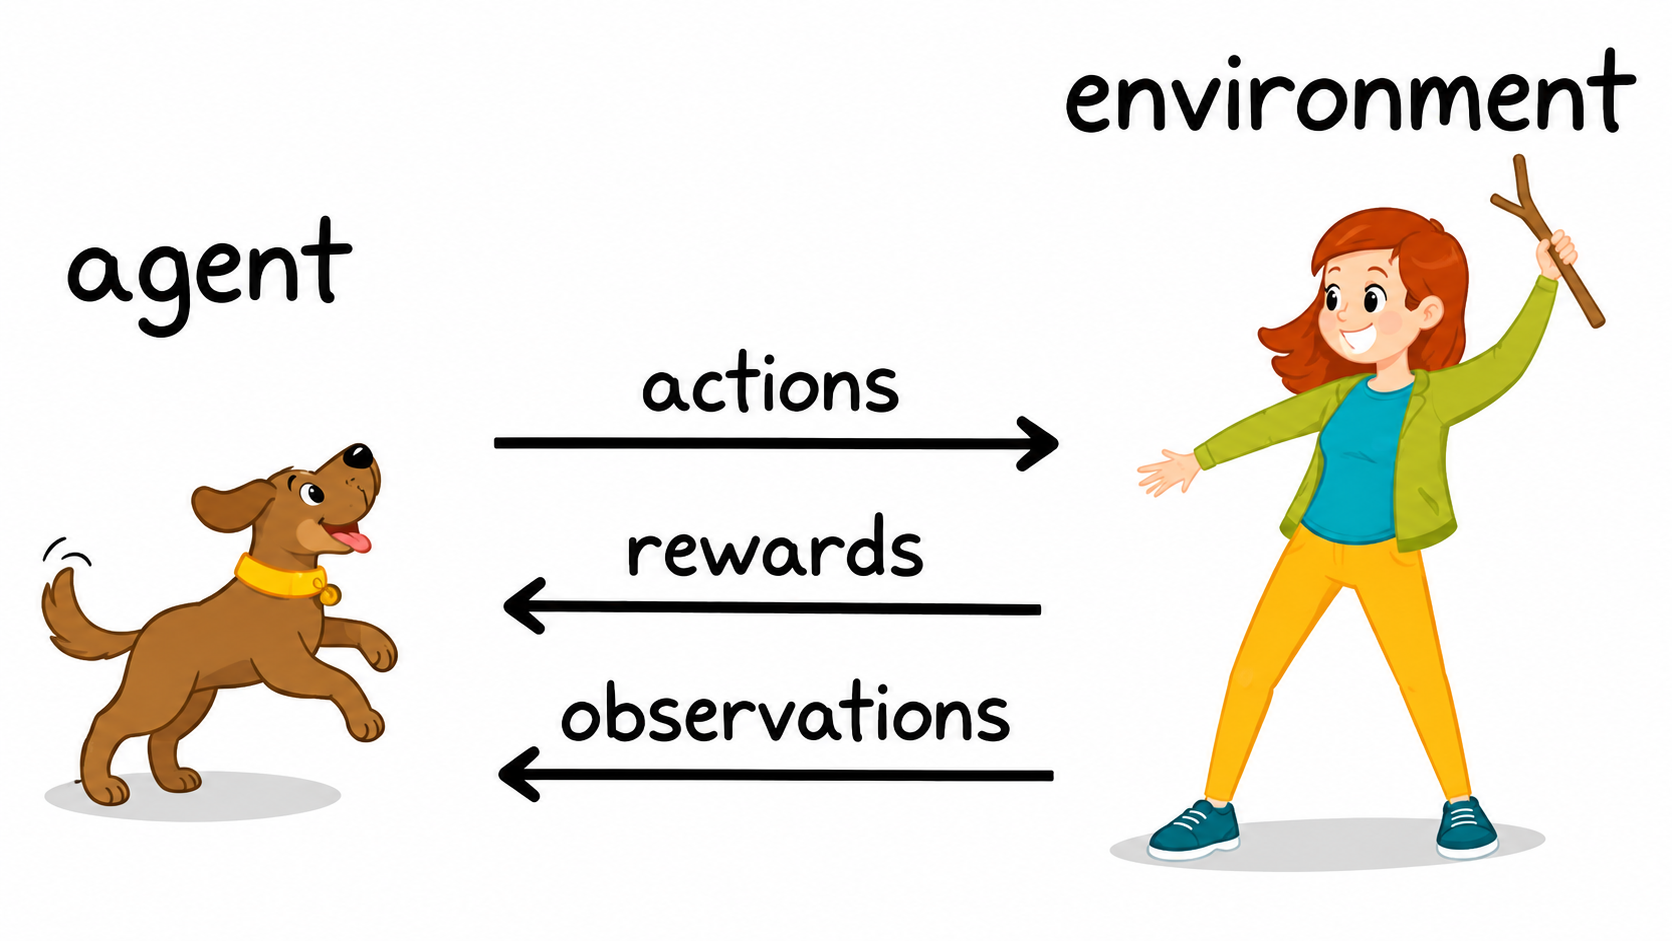
\includegraphics[width=0.5\textwidth]{images/RL_intro.png} 
\end{figure}
\noindent The agent has to:\begin{itemize}
    \item \textbf{Exploit}  what it has already experienced to obtain a reward.
    \item  \textbf{Explore} in order to make better action selections in the future.
\end{itemize}
One of the main challenges of reinforcement learning is the exploration-exploitation trade-off. On stochastic tasks, each action must be tried many times, in order to correctly estimate expected reward.
\section{Markov Decision Processes}
First of all we introduce a \textit{sequential} decision making approach. We see the agent that has to learn the policy, as an entity that can interact with the world/environment through actions $a_t$, and can receive by the environment an observation $o_t$ and a reward $r_t$ after each action. The agent interacts at discrete time steps, such discrete interaction generates a \textbf{trajectory} (or history) of tuples (observation-action-reward):\begin{equation}
    \underbrace{h_t}_{\text{history at time $t$}} = (o_0,a_0,r_1,o_1,a_1,r_2\dots, r_t,o_t,a_t).
\end{equation}
We define a state function $s_t=f(h_t)$ that describes the current state of the agent at time $t$ and depends on the history $h_t$ and is typically hidden or unknown.
\begin{boxdefinition}{Markov Assumption}{}
    A state $s_t$ is \textbf{Markovian} if the future is independent of the past information, given the present state: The probability of occurring in a given state $s_{t+1}$ by applying $a_t$ at time $t$, depend only on the current state $s_t$ and not on the history $h_t$:\begin{equation}
        \Prob(s_{t+1} \  |  \ s_t,a_t)=\Prob(s_{t+1} \  |  \ h_t,a_t).
    \end{equation}
\end{boxdefinition}
\noindent A state can always be made Markovian if we define the state exactly as the previous history:\begin{equation}
    s_t=h_t.
\end{equation}
In practice the current state is defined as the \textit{latest observation}:\begin{equation}
    s_t=o_t
\end{equation}
in this case the state is said to be \textbf{fully observable}.
\begin{figure}[H]
    \centering
    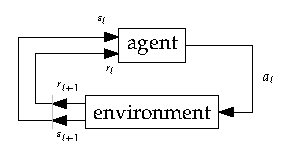
\includegraphics[width=0.5\textwidth]{images/MDP.eps} 
    \caption{Markov Decision Process scheme.}
    \label{MDP}
\end{figure}
A \textbf{Markov Decision Process (MDP)} is a sequential decision making scheme under the Markov assumption. The transition dynamics is generally stochastic: $\Prob(s_{t+1} \  |  \ s_t,a_t)$. An alternative notation to denote the fact that the next state is stochastic by applying $a_t$ on $s_t$ is the following:\begin{align}
    &s_{t+1}\sim \Prob(\cdot  \  |  \ s_t,a_t)\\
    \text{ or }\quad &s'\sim \Prob(\cdot  \  |  \ s,a)
\end{align}
A \textbf{reward} $r_t$ is a scalar signal representing feedback on the actions taken by the agent, and indicates how well an agent is doing at a given time step $t$. The reward is a function of the state and action (reward taken by applying a given action at a given state):\begin{equation}
    r_{t+1}=R(s_t,a_t).
\end{equation} 
We define the \textbf{cost} as the opposite of the reward. Although in reinforcement learning the objective is always to maximize the reward function, the fact that this is the best way to reach a goal is not guaranteed, in fact the so-called \textbf{Reward Hypothesis}:
\begin{quote}
``\textit{can all goals be achieved through the maximization of 
a numerical reward?}''
\end{quote}
remains an open question today.
\begin{boxdefinition}{Markov Decision Process}{MDP}
    An MDP is defined by a 5-tuple:\begin{equation}
        (S,A,\Prob,R,\gamma) 
    \end{equation}
    where:\begin{itemize}
        \item $S$ is the set of all possible states.
        \item $A$ is the set of all the actions the agent can take.
        \item $\Prob$ is the transition probability, which defines the dynamics of the environment.
        \item $R$ is the reward function.
        \item $\gamma$ is the \textbf{discount factor}, a real value within the interval $[0, 1]$ that determines the importance of future rewards compared to immediate ones.
    \end{itemize}
\end{boxdefinition}
\noindent The behavior of an agent is given by a policy, a function that determines how agents select actions.
\begin{boxdefinition}{Policy}{}
    A \textbf{policy} is a function $\pi:S\to A$ that assigns an action to every state.
\end{boxdefinition}
\noindent A policy can be deterministic:\begin{equation}
    \pi(s)=a
\end{equation}
\noindent or stochastic:\begin{equation}
    \pi(a \  |  \ s)\in [0,1] \quad \text{ with } \quad \sum_{a\in A}\pi(a \  |  \ s)=1.
\end{equation}
We can also write $a\sim \pi(\cdot  \  |  \  s)$. We can now define the \textbf{probability of a trajectory}: What's the probability of seeing a trajectory at time $t$ 
according to $\pi$ starting at $s_0$? We have the trajectory\begin{equation}
    (s_0,a_0,s_1\dots,s_t,a_t)
\end{equation}
and
\begin{align}
    &\Prob^\pi(s_0,a_0,s_1\dots,s_t,a_t)\\
    =& \pi(a_0 \  |  \ s_0)\Prob(s_1 \  |  \ s_0,a_0)\pi(a_1 \  |  \ s_1)\Prob(s_2 \  |  \ s_1,a_1)\dots 
    \Prob(s_t \  |  \ s_{t-1},a_{t-1})\pi(a_t \  |  \ s_t)
\end{align}
notice how we added $\pi$ as superscript to denote the fact that this probability depends on the given policy function. We can also define the \textbf{state visitation probability}, i.e. the probability of visiting a particular state $\hat s$ at time $t$ according to $\pi$ starting from $s_0$:\begin{equation}
    \Prob^\pi_t(s_t=\hat s \  |  \ s_0)=\sum_{a_0,s_1\dots a_{t-1}} \Prob^\pi(s_0,a_0,s_1\dots,s_t=\hat s).
\end{equation}
A basic example of a Markov decision process is a robotic manipulator with a hand gripper that can grab and carry a ball:\begin{itemize}
    \item the states are the possible robot configurations (joint values) and the ball position,
    \item the actions are the possible torques on the arm and the finger joints,
    \item the transition is stochastic, given by the physics (how the torques update the joint values over time) and by the noise,
    \item the policy maps each configuration+ball position to a torque for the joints,
    \item the cost (inverse of the reward) is the magnitude of the torque and the distance to the goal.
\end{itemize}
\subsection{MDP Horizon}
In Definition \ref{def:MDP} we introduced a discount factor $\gamma\in[0,1]$. This term weights the importance of immediate rewards with respect to future rewards:\begin{itemize}
    \item $\gamma=0$: Our agent only cares about immediate rewards.
    \item $\gamma=1$: Immediate and future rewards are equally important.
\end{itemize}
The discount factor is used in the \textbf{Value Function} $V^\pi$, a function that estimates the goodness of states and actions based on their value. It is also a measure to compare different policies.\begin{boxdefinition}{Value Function}{}
    The \textbf{Value Function} $V^\pi$ measures the cumulative reward (the sum of all future rewards, possibly discounted by the $\gamma$ factor) starting from $s_t$ and continuing to follow the policy $\pi$  for all subsequent actions. 
    \begin{align}
    V^\pi(s_t)=&\VA_\pi[r_{t+1}+\gamma r_{t+2}+\gamma^2 r_{t+3}+\gamma^3 r_{t+4}\dots  \  |  \  s_t]\\ 
    =&\VA\left[
        \sum_{h=0}^\infty \gamma^hr_{h+1}  \  |  \  s_0=s_t, a_h=\pi(s_h),s_{h+1}\sim \Prob(\cdot  \  |  \  s_h,a_h)
    \right].
\end{align}
\end{boxdefinition}
With $\VA$ we denote the expected value.
The Action-Value function $Q^\pi$ goes one step further than $V^\pi$, tying the value not only to the state, but also to the action you choose to take.
\begin{boxdefinition}{Action-Value Function}{}
    The \textbf{Action-Value Function} $Q^\pi$  measures the expected value of the cumulative return starting from a state $s_t$, performing a specific action $a_t$ and then continuing to follow the policy $\pi$.
    \begin{align}
    Q^\pi(s_t,a_t)=\VA\left[
         \sum_{h=0}^\infty\gamma^hr_h \  |  \ 
         (s_0,a_0)=(s_t,a_t), a_{h}=\pi(s_h), s_{h+1}\sim \Prob(\cdot \ | \ s_h,a_h)
    \right].
\end{align}
\end{boxdefinition}
\begin{boxtheorem}{The Bellman Equation}{}
    The value of a certain state can be expanded in terms of the 
current reward and the value of the next states according to 
the policy:\begin{equation}\label{Bellman_V}
    V^\pi(s_t)=\VA_\pi[r_t+\gamma r_{t+1}+\gamma^2 r_{t+2}+\gamma^3 r_{t+3}\dots  \  |  \  s_t]= 
    r_t+\gamma \VA_{s_{t+1}\sim \Prob(\cdot \ | \ s_t,\greenText{ \pi(s_t)})}[V^\pi(s_{t+1})].
\end{equation}
\end{boxtheorem}
\noindent The Bellman equation can be applied to the action-value function:\begin{equation}\label{Bellman_Q}
    Q^\pi(s_t,\greenText{a_t})=r_t+\gamma\VA_{s_{t+1}\sim \Prob(\cdot \ | \ s_t,\greenText{ a_t})}[V^\pi(s_{t+1})]
\end{equation}
In Equation \eqref{Bellman_V} $r$ is a function of $s$ and $\pi(s)$ while in equation \eqref{Bellman_Q} it is a function of $s$ and $a$ (as highlighted by the \greenText{ green } characters). As a result of these equations we have the following identity:
\begin{equation}
    V^\pi(s)=Q^\pi(s,\pi(s))
\end{equation}
$V^\pi$ can be expressed in terms of $Q^\pi$.
\end{document}